\documentclass[portrait,final,a0paper]{baposter}
%\documentclass[a4shrink,portrait,final]{baposter}
% Usa a4shrink for an a4 sized paper.

\tracingstats=2

\usepackage{calc}
\usepackage{graphicx}
\usepackage{amsmath}
\usepackage{amssymb}
\usepackage{relsize}
\usepackage{multirow}
\usepackage{bm}

\usepackage{graphicx}
\usepackage{multicol}

\usepackage{pgfbaselayers}
\pgfdeclarelayer{background}
\pgfdeclarelayer{foreground}
\pgfsetlayers{background,main,foreground}

\usepackage{times}
\usepackage{helvet}
%\usepackage{bookman}
\usepackage{palatino}
% \usepackage{tikz}
% \usetikzlibrary{arrows,decorations.pathmorphing,backgrounds,positioning,fit,shadows}

\newcommand{\captionfont}{\footnotesize}

\selectcolormodel{cmyk}

\graphicspath{{images/}}

%%%%%%%%%%%%%%%%%%%%%%%%%%%%%%%%%%%%%%%%%%%%%%%%%%%%%%%%%%%%%%%%%%%%%%%%%%%%%%%%
%%%% Some math symbols used in the text
%%%%%%%%%%%%%%%%%%%%%%%%%%%%%%%%%%%%%%%%%%%%%%%%%%%%%%%%%%%%%%%%%%%%%%%%%%%%%%%%
% Format 
\newcommand{\Matrix}[1]{\begin{bmatrix} #1 \end{bmatrix}}
\newcommand{\Vector}[1]{\Matrix{#1}}
\newcommand*{\SET}[1]  {\ensuremath{\mathcal{#1}}}
\newcommand*{\MAT}[1]  {\ensuremath{\mathbf{#1}}}
\newcommand*{\VEC}[1]  {\ensuremath{\bm{#1}}}
\newcommand*{\CONST}[1]{\ensuremath{\mathit{#1}}}
\newcommand*{\norm}[1]{\mathopen\| #1 \mathclose\|}% use instead of $\|x\|$
\newcommand*{\abs}[1]{\mathopen| #1 \mathclose|}% use instead of $\|x\|$
\newcommand*{\absLR}[1]{\left| #1 \right|}% use instead of $\|x\|$

\def\norm#1{\mathopen\| #1 \mathclose\|}% use instead of $\|x\|$
\newcommand{\normLR}[1]{\left\| #1 \right\|}% use instead of $\|x\|$

%%%%%%%%%%%%%%%%%%%%%%%%%%%%%%%%%%%%%%%%%%%%%%%%%%%%%%%%%%%%%%%%%%%%%%%%%%%%%%%%
% Multicol Settings
%%%%%%%%%%%%%%%%%%%%%%%%%%%%%%%%%%%%%%%%%%%%%%%%%%%%%%%%%%%%%%%%%%%%%%%%%%%%%%%%
\setlength{\columnsep}{0.7em}
\setlength{\columnseprule}{0mm}


%%%%%%%%%%%%%%%%%%%%%%%%%%%%%%%%%%%%%%%%%%%%%%%%%%%%%%%%%%%%%%%%%%%%%%%%%%%%%%%%
% Save space in lists. Use this after the opening of the list
%%%%%%%%%%%%%%%%%%%%%%%%%%%%%%%%%%%%%%%%%%%%%%%%%%%%%%%%%%%%%%%%%%%%%%%%%%%%%%%%
\newcommand{\compresslist}{%
\setlength{\itemsep}{1pt}%
\setlength{\parskip}{0pt}%
\setlength{\parsep}{0pt}%
}


%%%%%%%%%%%%%%%%%%%%%%%%%%%%%%%%%%%%%%%%%%%%%%%%%%%%%%%%%%%%%%%%%%%%%%%%%%%%%%
%%% Begin of Document
%%%%%%%%%%%%%%%%%%%%%%%%%%%%%%%%%%%%%%%%%%%%%%%%%%%%%%%%%%%%%%%%%%%%%%%%%%%%%%

\begin{document}

%%%%%%%%%%%%%%%%%%%%%%%%%%%%%%%%%%%%%%%%%%%%%%%%%%%%%%%%%%%%%%%%%%%%%%%%%%%%%%
%%% Here starts the poster
%%%---------------------------------------------------------------------------
%%% Format it to your taste with the options
%%%%%%%%%%%%%%%%%%%%%%%%%%%%%%%%%%%%%%%%%%%%%%%%%%%%%%%%%%%%%%%%%%%%%%%%%%%%%%
% Define some colors
\definecolor{silver}{cmyk}{0,0,0,0.3}
\definecolor{yellow}{cmyk}{0,0,0.9,0.0}
\definecolor{reddishyellow}{cmyk}{0,0.22,1.0,0.0}
\definecolor{black}{cmyk}{0,0,0.0,1.0}
\definecolor{darkYellow}{cmyk}{0,0,1.0,0.5}
\definecolor{darkSilver}{cmyk}{0,0,0,0.1}

\definecolor{lightyellow}{cmyk}{0,0,0.3,0.0}
\definecolor{lighteryellow}{cmyk}{0,0,0.1,0.0}
\definecolor{lighteryellow}{cmyk}{0,0,0.1,0.0}
\definecolor{lightestyellow}{cmyk}{0,0,0.05,0.0}

%%
\typeout{Poster Starts}
\background{
  \begin{tikzpicture}[remember picture,overlay]%
    \draw (current page.north west)+(-2em,2em) node[anchor=north west] {
\includegraphics[height=1.1\textheight]{silhouettes_background}};
  \end{tikzpicture}%
}

\newlength{\leftimgwidth}
\begin{poster}%
  % Poster Options
  {
  % Show grid to help with alignment
  grid=no,
  % Column spacing
  colspacing=1em,
  % Color style
  bgColorOne=lighteryellow,
  bgColorTwo=lightestyellow,
  borderColor=reddishyellow,
  headerColorOne=yellow,
  headerColorTwo=reddishyellow,
  headerFontColor=black,
  boxColorOne=lightyellow,
  boxColorTwo=lighteryellow,
  % Format of textbox
  textborder=roundedleft,
%  textborder=rectangle,
  % Format of text header
  eyecatcher=yes,
  headerborder=open,
  headerheight=0.08\textheight,
  headershape=roundedright,
  headershade=plain,
  headerfont=\Large\textsf, %Sans Serif
  boxshade=none,
%  background=shade-tb,
  background=plain,
  linewidth=2pt
  }
  % Eye Catcher
  {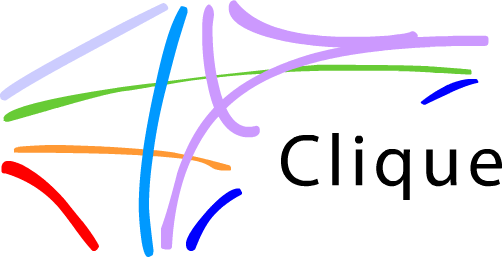
\includegraphics[width=10em]{clique}} % No eye catcher for this poster. (eyecatcher=no above). If an eye catcher is present, the title is centered between eye-catcher and logo.
  % Title
  {\sf %Sans Serif
  %\bf% Serif
  Clustering networks with the collapsed SBM}
  % Authors
  {\sf %Sans Serif
  % Serif
  %\vspace{1em}
  Aaron F. McDaid, Brendan Murphy, Nial Friel and Neil Hurley
  }
  % University logo
  {% The makebox allows the title to flow into the logo, this is a hack because of the L shaped logo.
    \makebox[8em][r]{%
      \begin{minipage}{16em}
        \hfill
        
\includegraphics[height=7.0em]{sfi_trans}
      \end{minipage}
    }
  }

  \tikzstyle{light shaded}=[top color=baposterBGtwo!30!white,bottom color=baposterBGone!30!white,shading=axis,shading angle=30]

  % Width of left inset image
     \setlength{\leftimgwidth}{0.78em+8.0em}

%%%%%%%%%%%%%%%%%%%%%%%%%%%%%%%%%%%%%%%%%%%%%%%%%%%%%%%%%%%%%%%%%%%%%%%%%%%%%%
%%% Now define the boxes that make up the poster
%%%---------------------------------------------------------------------------
%%% Each box has a name and can be placed absolutely or relatively.
%%% The only inconvenience is that you can only specify a relative position 
%%% towards an already declared box. So if you have a box attached to the 
%%% bottom, one to the top and a third one which should be in between, you 
%%% have to specify the top and bottom boxes before you specify the middle 
%%% box.
%%%%%%%%%%%%%%%%%%%%%%%%%%%%%%%%%%%%%%%%%%%%%%%%%%%%%%%%%%%%%%%%%%%%%%%%%%%%%%
    %
    % A coloured circle useful as a bullet with an adjustably strong filling
    \newcommand{\colouredcircle}[1]{%
      \tikz{\useasboundingbox (-0.2em,-0.32em) rectangle(0.2em,0.32em); \draw[draw=black,fill=baposterBGone!80!black!#1!white,line width=0.03em] (0,0) circle(0.18em);}}

%%%%%%%%%%%%%%%%%%%%%%%%%%%%%%%%%%%%%%%%%%%%%%%%%%%%%%%%%%%%%%%%%%%%%%%%%%%%%%
  \headerbox{Contribution}{name=contribution,column=0,row=0}{
%%%%%%%%%%%%%%%%%%%%%%%%%%%%%%%%%%%%%%%%%%%%%%%%%%%%%%%%%%%%%%%%%%%%%%%%%%%%%%
   {}We take the Stochastic Block Model of Nowicki \& Snijders (2001) and create a fast
   MCMC algorithm. A network is input to the algorithm and the output is
   a sample of clusterings of the nodes.
   We employ \emph{collapsing} to integrate out variables that are not of
   interest, and we use recent innovative moves in our algorithm.
   We also allow that the number of clusters, $K$, in an output of the
   algorithm rather than an input to the algorithm.
   We should that it can accurately estimate the number of clusters in synthetic
   data and demonstrate the model on real data.
  \vspace{0.3em}
 }

%%%%%%%%%%%%%%%%%%%%%%%%%%%%%%%%%%%%%%%%%%%%%%%%%%%%%%%%%%%%%%%%%%%%%%%%%%%%%%
  \headerbox{Model}{name=model,column=0,below=contribution}{
%%%%%%%%%%%%%%%%%%%%%%%%%%%%%%%%%%%%%%%%%%%%%%%%%%%%%%%%%%%%%%%%%%%%%%%%%%%%%%

$N$, the number of nodes in the network, is given. This factor diagram shows the
relationships between the variables in the standard SBM.


\centering
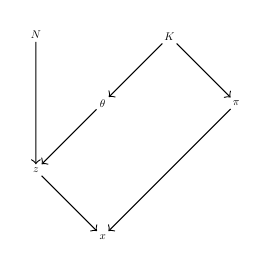
\begin{tikzpicture}[scale=0.4, transform shape]
\tikzstyle{var}=[node distance=3cm, inner sep=0.1cm]
	\node[var] (K) {$K$};
	\node[var, below right of=K] (pi) {$\pi$};
	\node[var, below left of=K] (theta) {$\theta$};
	% \node[node distance=3cm, above left of=theta] (dirichlet) {$\mbox{Dirichlet}(\alpha)$};
	% \node[node distance=3cm, above right of=pi] (beta) {$\mbox{Beta}(\beta_1,\beta_2)$};
	\node[var, below left of=theta] (z) {$ z $};
	\node[var, below right of=z] (x) {$x$};
	\node[var, node distance=4.3cm, above of=z] (N) {$N$};

	\draw[->] (K) -- (pi) ;
	\draw[->] (K) -- (theta) ;
	\draw[->] (N) -- (z) ;
	\draw[->] (theta) -- (z) ;
	\draw[->] (z) -- (x) ;
	\draw[->] (pi) -- (x) ;
\end{tikzpicture}

$K$ and $N$ are inputs. The network, $x$, is at the bottom.
\begin{itemize}
	\item $\pi$ is a $K \times K$ matrix; $\pi_{ij} \sim \mbox{Beta}(\beta_1, \beta_2)$
	\item $\theta$ is a vector of length $K$; $\theta \sim \mbox{Dirichlet}(\alpha)$
	\item $z$ is a vector of length $N$ %; $z_n \sim \mbox{Multinomial}(\theta)$
	\item $x$ is a $N \times N$ matrix, the adjacency matrix.
\end{itemize}
We also allow $K$ to be an output, by specifying a prior for $K$. $K \sim \mbox{Poisson}(1)$.


  \vspace{0.3em}
  }

%%%%%%%%%%%%%%%%%%%%%%%%%%%%%%%%%%%%%%%%%%%%%%%%%%%%%%%%%%%%%%%%%%%%%%%%%%%%%%
  \headerbox{Bayes' Theorem}{name=fitting,column=0,below=model}{
%%%%%%%%%%%%%%%%%%%%%%%%%%%%%%%%%%%%%%%%%%%%%%%%%%%%%%%%%%%%%%%%%%%%%%%%%%%%%%
  Users will have a network, $x$, of $N$ nodes. The aim is to estimate $z$, the clustering,
  and estimate the number of clusters.
  We draw from $$ K, z | x, N $$
  whereas the original SBM of Nowicki \& Snijders draws from
  $$ z, \theta, \pi | x, N, K $$
  We don't usually care about $\theta$ and $\pi$.

  $$
  \mathrm{P}(K,z|x,N) \propto \mathrm{P}(K) \mathrm{P}(z|K,N) \mathrm{P}(x|z,K,N)
  $$
  \vspace{0.3em}
  }

%%%%%%%%%%%%%%%%%%%%%%%%%%%%%%%%%%%%%%%%%%%%%%%%%%%%%%%%%%%%%%%%%%%%%%%%%%%%%%
  % \headerbox{Distance Measure}{name=measure,column=0,below=fitting}{
%%%%%%%%%%%%%%%%%%%%%%%%%%%%%%%%%%%%%%%%%%%%%%%%%%%%%%%%%%%%%%%%%%%%%%%%%%%%%%
   % The Mahalanobis angle between the identity coefficients $\VEC{\alpha_{n}}$
   % was used for classification.
  % \vspace{0.3em}
  % }

%%%%%%%%%%%%%%%%%%%%%%%%%%%%%%%%%%%%%%%%%%%%%%%%%%%%%%%%%%%%%%%%%%%%%%%%%%%%%%
  \headerbox{Estimating the number of clusters}{name=results neutralization,column=1,row=0,span=1}{
%%%%%%%%%%%%%%%%%%%%%%%%%%%%%%%%%%%%%%%%%%%%%%%%%%%%%%%%%%%%%%%%%%%%%%%%%%%%%%
  With our prior on $K$, and using Markov moves from the algorithm in Nobile \& Fearnside (2007), we estimate the number of clusters in the same way we estimate the assignments. The algorithm searches over the space of all clusterings, regardless of $K$.

  \textbf{Synthetic data}

  For a given number of clusters, $K$, a directed network is generated with 10 nodes in each clusters. For each of the $K \times $ blocks, the expected density, $\pi_{ij}$ is drawn from $ \mbox{Beta}(1,1) \equiv \mbox{Uniform}(0,1) $.

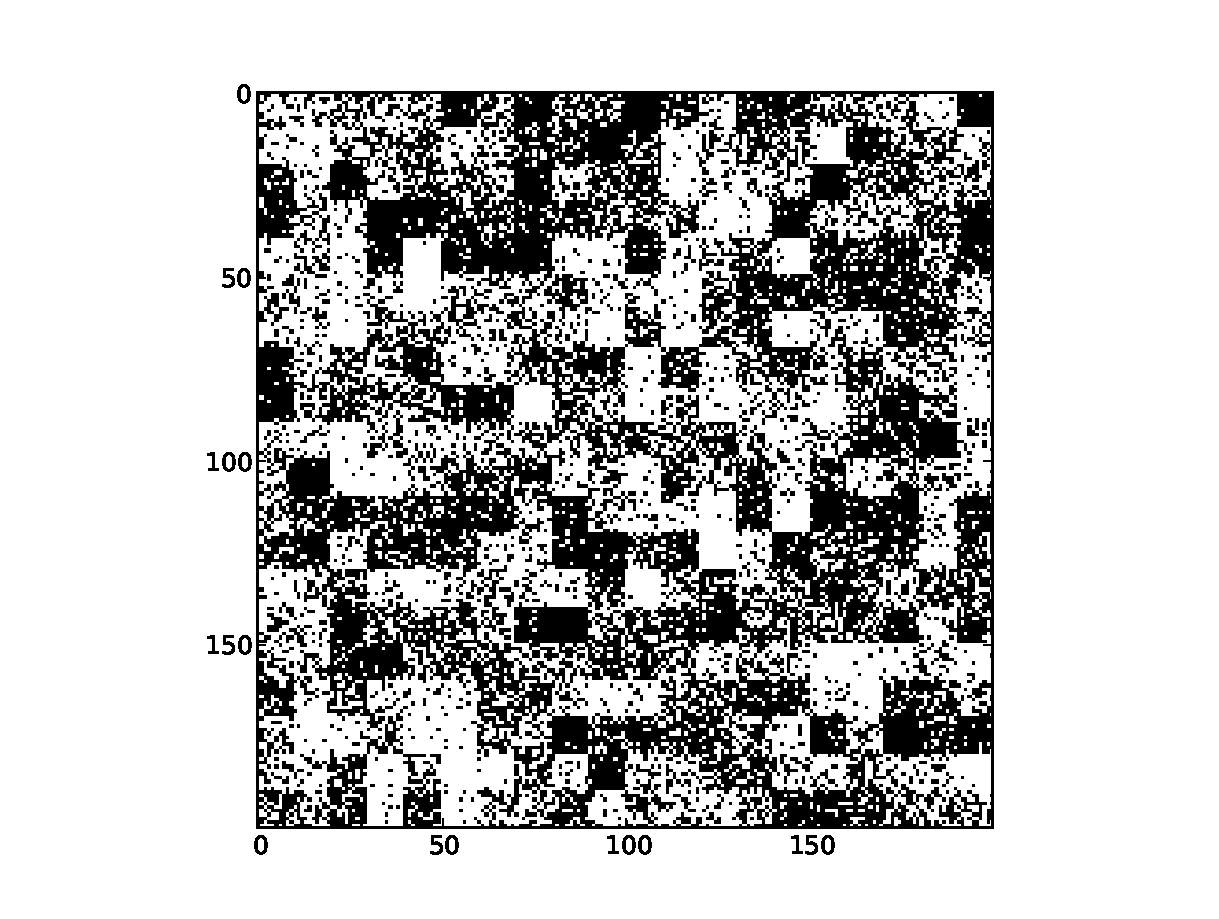
\includegraphics[width=19em]{K20adjacency}

  \textbf{Results}

  The black lines represent 10 different experiments, where synthetic networks were generated with 5, 10, \ldots 50 clusters. The algorithm arrives at the correct answer typically in 1,000 - 10,000 iterations.

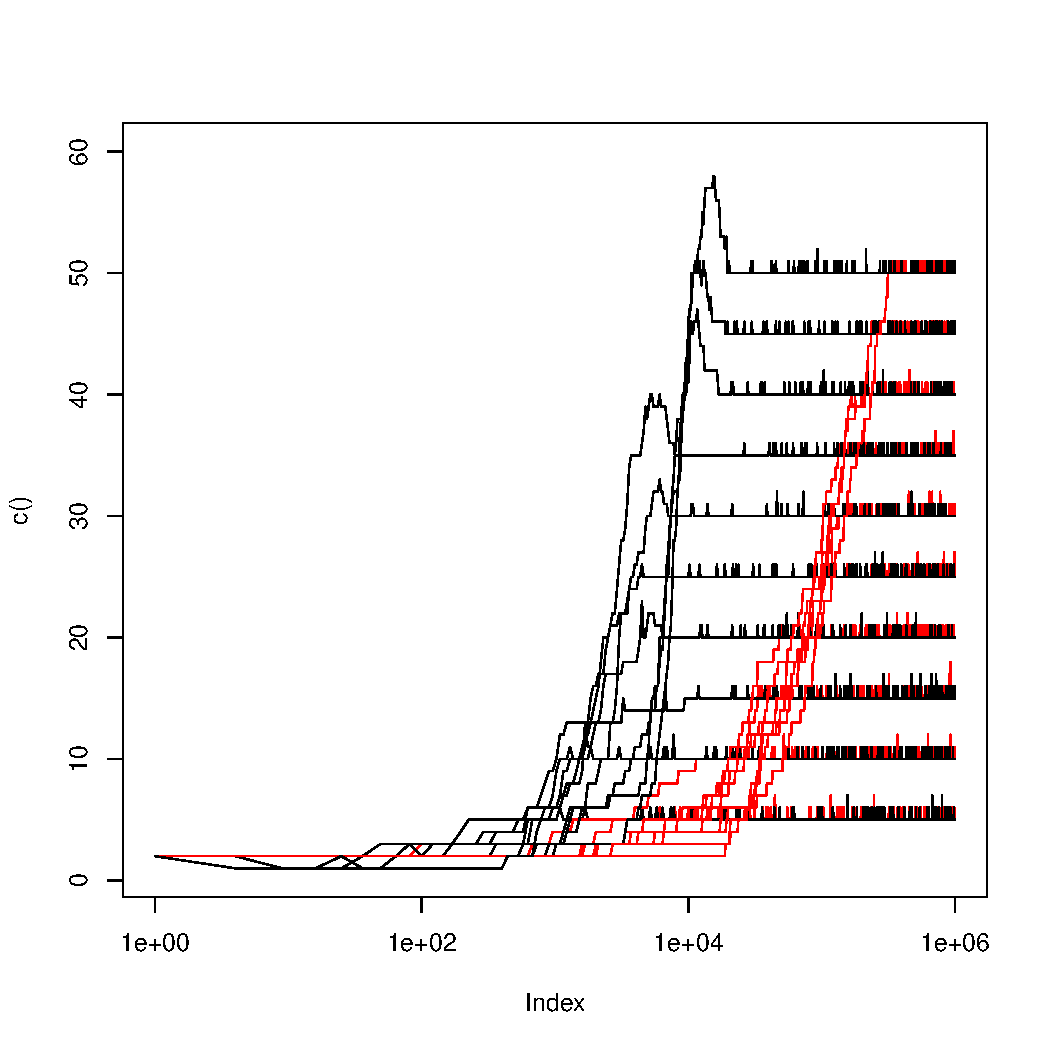
\includegraphics[width=22em]{LazSynthK}
  %\vspace{0.5em}
  }
%%%%%%%%%%%%%%%%%%%%%%%%%%%%%%%%%%%%%%%%%%%%%%%%%%%%%%%%%%%%%%%%%%%%%%%%%%%%%%
  \headerbox{Funding}{name=funding,column=1,span=2,above=bottom}{
%%%%%%%%%%%%%%%%%%%%%%%%%%%%%%%%%%%%%%%%%%%%%%%%%%%%%%%%%%%%%%%%%%%%%%%%%%%%%%
  \smaller 
  \hspace{1em}This work was carried out in the CLIQUE Strategic Research
  Cluster which is funded by Science Foundation Ireland (SFI)
  under grant number 08/SRC/I1407.

  }
%%%%%%%%%%%%%%%%%%%%%%%%%%%%%%%%%%%%%%%%%%%%%%%%%%%%%%%%%%%%%%%%%%%%%%%%%%%%%%
  \headerbox{Application to survey network}{name=results,column=2,row=0}{
%%%%%%%%%%%%%%%%%%%%%%%%%%%%%%%%%%%%%%%%%%%%%%%%%%%%%%%%%%%%%%%%%%%%%%%%%%%%%%
	      We did a survey of the participants of the \emph{Web Science Summer School 2011} hosted in DERI, Galway. 74 participants were asked who they knew before the summer school and also who they talked to at the summer school. 41 responded. We created an unweighted directed network and fed it into our SBM algorithm. There was an edge from A to B if A reported having either kind of link with B. We included the non-respondents - they have no edges coming out of them, but they do have edges coming in.
      \mbox{\hspace{0.3\linewidth}\rule{0.4\linewidth}{1pt}\hspace{0.3\linewidth}}\\

      Our algorithm divides the 74 people into 7 clusters. The seven clusters were interpretable, one of the DERI students assisted us in interpreting the groups. The \emph{non-respondents} were identified, but split into two clusters. The algorithm divided them in two due to differences in the connections coming into these two subgroups.

      The \emph{organizers} were connected, in both directions, with the vast majority of participants, as expected.

      The \emph{visitors} were people from outside DERI who attended the summer school.


      The \emph{locals} include other people at DERI who attended the Summer School but were not part of organizing.

      Finally, there was a small cluster we've called \emph{Quiet}, which seem to be distinguished simply by having low in-degree and low out-degree.

  {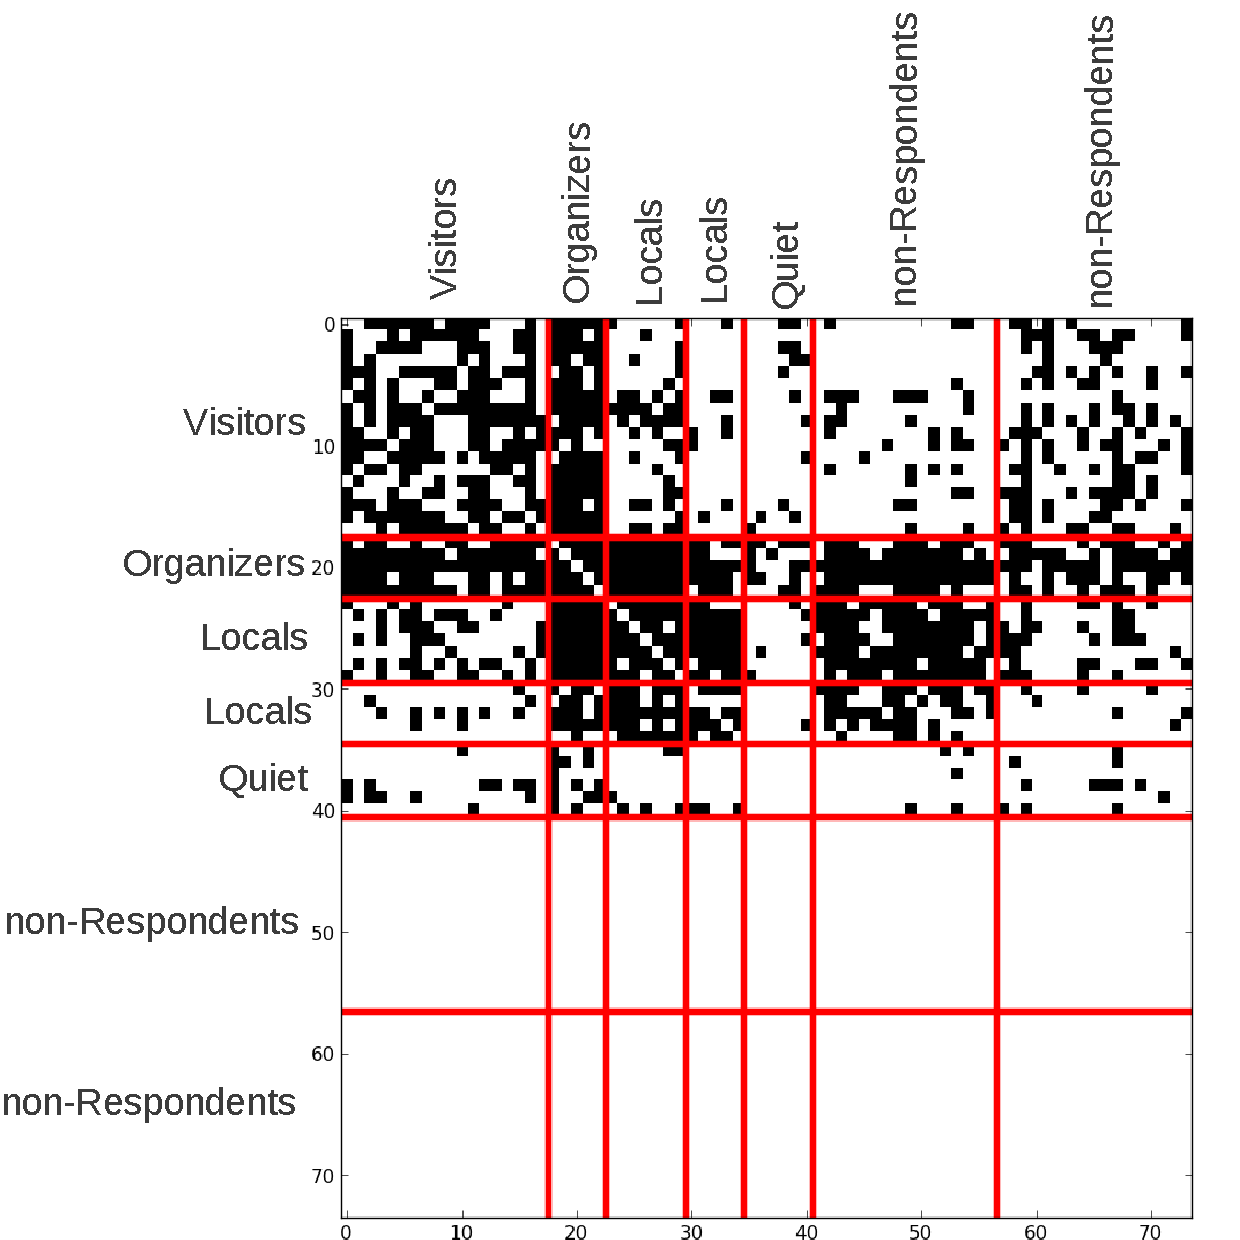
\includegraphics[width=20em]{labelled_survey_adj}}

  \\
  \vspace{0.5em}
  }
  \headerbox{What is collapsing?}{name=collapsing,column=1,span=2,below=results}{
  One option would have been to draw from
  $$ K, z, \theta, \pi | x, N $$
  i.e. given a network and the number of nodes, draw the clustering alongside the estimates for the real-valued variables $\pi$ and $\theta$.
  This would have been difficult to implement, requiring some form of Reversible Jump Markov Chain Monte Carlo (RJMCMC), and would also
  likely have been quite inefficient.
  Given that we are not interested in $\pi$ and $\theta$, we can use the following identity:
  $$ \mathrm{P}(K, z | x, N) = \int \mathrm{d}\pi \; \mathrm{d}\theta \; \mathrm{P}(K, z, \theta, \pi | x, N) $$
  This is straightforward to solve analytically in this model, hence giving us a simpler expression for our desired estimator.
  $$ \mathrm{P}(K, z | x, N) $$
  }

%%%%%%%%%%%%%%%%%%%%%%%%%%%%%%%%%%%%%%%%%%%%%%%%%%%%%%%%%%%%%%%%%%%%%%%%%%%%%%

%%%%%%%%%%%%%%%%%%%%%%%%%%%%%%%%%%%%%%%%%%%%%%%%%%%%%%%%%%%%%%%%%%%%%%%%%%%%%%
  \headerbox{References}{name=references,column=0,above=bottom}{
%%%%%%%%%%%%%%%%%%%%%%%%%%%%%%%%%%%%%%%%%%%%%%%%%%%%%%%%%%%%%%%%%%%%%%%%%%%%%%
    \smaller
    \vspace{-0.4em}
    \bibliographystyle{ieee}
    \renewcommand{\section}[2]{\vskip 0.05em}
      \begin{thebibliography}{1}\itemsep=-0.01em
      \setlength{\baselineskip}{0.4em}
      \bibitem{amberg07:nonrigid}
        B.~Amberg, S.~Romdhani, T. Vetter.
        \newblock {O}ptimal {S}tep {N}onrigid {ICP} {A}lgorithms for {S}urface {R}egistration
        \newblock In {\em Computer Vision and Pattern Recognition 2007}
      \bibitem{amberg08:recognition}
        B.~Amberg, R.~Knothe, T. Vetter.
        \newblock Expression Invariant Face Recognition with a 3D Morphable Model
        \newblock In {\em Automated Face and Gesture Recognition 2008}
      \end{thebibliography}
  }
%%%%%%%%%%%%%%%%%%%%%%%%%%%%%%%%%%%%%%%%%%%%%%%%%%%%%%%%%%%%%%%%%%%%%%%%%%%%%%
  %\headerbox{Open Questions}{name=questions,column=0,span=1,below=fitting,above=references}{
%%%%%%%%%%%%%%%%%%%%%%%%%%%%%%%%%%%%%%%%%%%%%%%%%%%%%%%%%%%%%%%%%%%%%%%%%%%%%%
    %While the expression and identity space are linearly independent, there is
    %some expression left in the identity model. This is because a ``neutral''
    %face is interpreted differently by the subjects.
%
    %We investigate learning ``pure'' separated models from our the available ``impure'' data.
  %}

\end{poster}

\end{document}
